\chapter{The chain of custody}\label{ch:chain}

\section{What the chain is}

The Cellular Performance Gauge is a chain of stages that takes a specimen's raw array files and returns, for every cell found in it, a reading $A$ with its
interval and tier. Its Standard Operating Procedure walks every step; its Operations Manual gives the constants and the rulings; both are regenerated from the
code on every change, so that neither can describe a stage the code does not run. This chapter is the reader's walk through the chain, stage by stage
(Figure~\ref{fig:chain}).

\begin{figure}[t]\centering
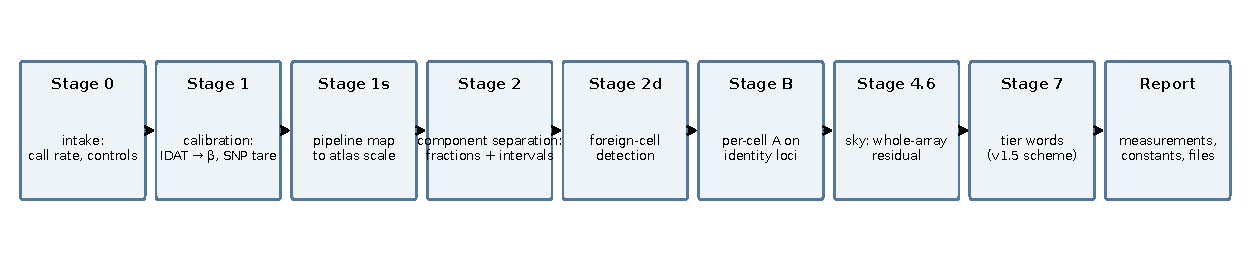
\includegraphics[width=\textwidth]{figures/part4/fig_chain_flow.pdf}
\caption{The chain of custody, from intake to report.}
\label{fig:chain}
\end{figure}

\section{Stage 0: intake}

The specimen's IDAT pair is opened and its own quality numbers are read: detection call rate, control-probe intensities, bisulfite-conversion controls,
SNP-probe clusters. Below a call rate of 0.93 the specimen is quarantined and no report is written; between 0.93 and 0.98 it proceeds with a flag. Input that
arrives as $\beta$ values without the raw files can be read, but every output then carries \texttt{intake\_verified: False} and one printed line saying so.

\section{Stage 1: calibration}

Background and dye-bias correction and probe-type handling produce $\beta$ at every probe. Probes indistinguishable from background are removed before any later
stage sees a $\beta$ (Chapter~\ref{ch:instrument}). Stage~1 returns, beside $\beta$, the array's detection numbers, control intensities and SNP-probe noise, so that
later stages can use the array's own measurements of itself. The commissioned chain then maps $\beta$ onto the first atlas's scale with the
per-pipeline map of Chapter~\ref{ch:instrument}; on the second atlas no map is applied, because Stage~1's output is already on the atlas scale.

\section{Stage 2: composition}

The specimen is separated into cells: on the first atlas by the commissioned solver, with a second, blind solver beside it as a cross-check; on the
second atlas by the v2 solver with the candidate set for the specimen type (Chapter~\ref{ch:separation}). The output is a fraction and a bootstrap
interval for every candidate cell and a present or absent call.

\section{Stage 2d: cells that should not be there}

Non-blood templates are fitted jointly with blood. A non-blood cell in whole blood is reported only when detected. The composition check also decides whether the
specimen is the whole blood it was labelled; when it is not, cell tiers are withheld.

\section{The reading}

Every cell found present is read on its own identity loci, Eq.~\eqref{eq:A} (the first atlas's per-cell identity sets, or v2's), divided by its class floor, with a bootstrap interval over loci. A cell whose fraction is
too small to score confidently is printed without a tier word. Flags travel with every reading that needs them: a sequencing-only identity set, a single pooled
sample, an assumed source term, a low call rate.

\section{The sky and the out-of-span map}

The whole-array residual is drawn as the sky (Chapter~\ref{ch:sky}). The out-of-span map, when adopted, is drawn beside it.

\section{Tier words}

The continuous reading is given its word from the tier scheme in force, and nothing else changes it: no age, no laboratory, no population.

\section{Serial mode}

When an earlier draw of the same person is supplied, the chain adds per-cell differences, the difference sky and, with three or more draws, a trajectory
(Chapter~\ref{ch:serial}).

\section{The report bundle}

The report is a set of tabs rendered from one bundle that records every input file with its checksum, every constant with its source file, and every stage's
output. Its vocabulary is guarded at render time (Chapter~\ref{ch:report}). A run is named by date and sequence and never overwrites another.

\section{Which atlas the chain runs on}

The commissioned chain runs on the first atlas. The second atlas and its reader run as a separate preview until its acceptance tests pass: held-out
transfer of identity loci, known-mixture composition, the out-of-span tests and a same-cell comparison between atlases. Then the switch-over replaces the first
atlas in one change. Until then, every reading on the second atlas is labeled \preview{} (Chapter~\ref{ch:firstreadings}).

\section{Documents the chain generates about itself}

\begin{itemize}
\item the chain sequence, derived from the conductor's calls, so a stage cannot be listed that the code does not run;
\item the inventory of every runtime file with its role;
\item the Standard Operating Procedure, whose generated sections and status banners come from the code;
\item the Operations Manual, built as a PDF from its data file;
\item a fresh reference report from one repository array, and the report-tab reference derived from that render.
\end{itemize}
The rule behind all of them: a document that describes the instrument is rebuilt from the instrument, never edited to match it.
